\documentclass{article}

\usepackage{tikz}
\usepackage{tikz}
\usepackage{pgfplots}
\usetikzlibrary{backgrounds, positioning, fit}
\usetikzlibrary{shapes.geometric}
\usetikzlibrary{patterns}

%% put tikzlibrary below if necessary

% set up externalization
\usetikzlibrary{external}
\tikzset{external/system call={latex \tikzexternalcheckshellescape -halt-on-error
-interaction=batchmode -jobname "\image" "\texsource";
dvips -o "\image".ps "\image".dvi;
ps2eps "\image.ps"}}
\tikzexternalize



\begin{document}


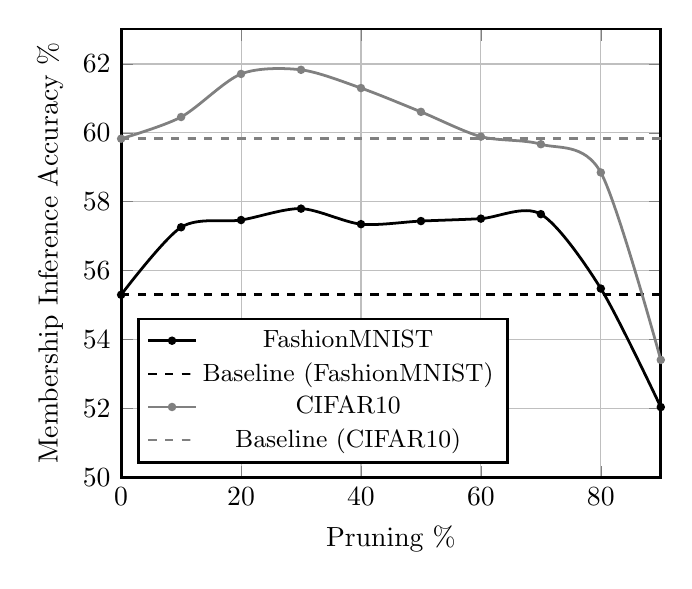
\begin{tikzpicture}
\begin{axis}[
%title={(a) FashionMNIST \& CIFAR10},
%title style={at={(0.5,0)},anchor=north,yshift=-40, font=\LARGE},
legend style={font=\small},
legend pos =  south west,
line width=1.0pt,
mark size=1.0pt,
ymin=50,
xmin=0,
xmax=90,
legend entries={FashionMNIST, Baseline (FashionMNIST), CIFAR10, Baseline (CIFAR10)},
ylabel={Membership Inference Accuracy \%},
xlabel={Pruning \%},
xlabel near ticks,
ylabel near ticks,
% extra x ticks={1,10,...,400},
% extra y ticks={0,0.5,...,10},
% extra y tick labels={},
% extra x tick labels={},
% extra x tick style={grid=major},
% extra y tick style={grid=major},
grid=major
]
\addplot[
    color=black,
    solid,
    mark=*,
    mark options={solid},
    smooth
    ]
    coordinates {
    (0,55.30)(10,57.26)(20,57.47)(30,57.80)(40,57.35)(50,57.44)(60,57.51)(70,57.64)(80,55.48)(90,52.04)
      };
\addplot[
    color=black,
    dashed,
    smooth
    ]
    coordinates {
    (0,55.30)(10,55.30)(20,55.30)(30,55.30)(40,55.30)(50,55.30)(60,55.30)(70,55.30)(80,55.30)(90,55.30)
      };
\addplot[
    color=gray,
    solid,
    mark=*,
    mark options={solid},
    smooth
    ]
    coordinates {
    (0,59.83)(10,60.46)(20,61.71)(30,61.83)(40,61.30)(50,60.61)(60,59.89)(70,59.67)(80,58.85)(90,53.41)
      };
\addplot[
    color=gray,
    dashed,
    smooth
    ]
    coordinates {
    (0,59.83)(10,59.83)(20,59.83)(30,59.83)(40,59.83)(50,59.83)(60,59.83)(70,59.83)(80,59.83)(90,59.83)
      };
\end{axis}
\end{tikzpicture}


\end{document}
